
In the discrete representation, frequently, it is necessary to resample or
evaluate the data, or its derivatives, at points within the domain range,
different that the original pairs $\{(t_j, y_j)\}$ at which our observations
have been measured. An example of this it is shown in the figure
\ref{FIG:RESAMPLE}. For this purpose interpolation is used.
This allows to treat each functional datum as a single entity $f(t)$, which
varies continuously throughout $t$.

\begin{figure}[Function resampled using interpolation]{FIG:RESAMPLE}{Function resampled using interpolation}

  \subfigure[SBFIG:RESAMPLE1]{Original observation}{
  	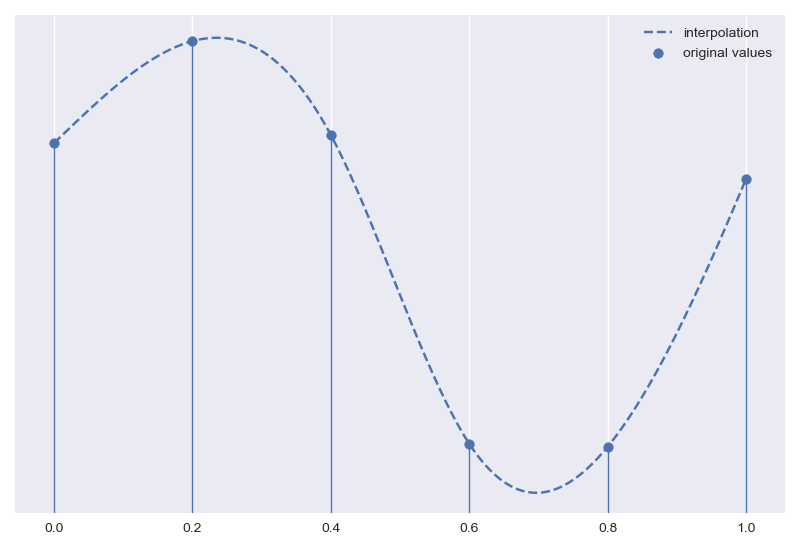
\includegraphics[width=7.5cm]{original-function}} \quad
  \subfigure[SBFIG:RESAMPLE2]{Observation resampled}{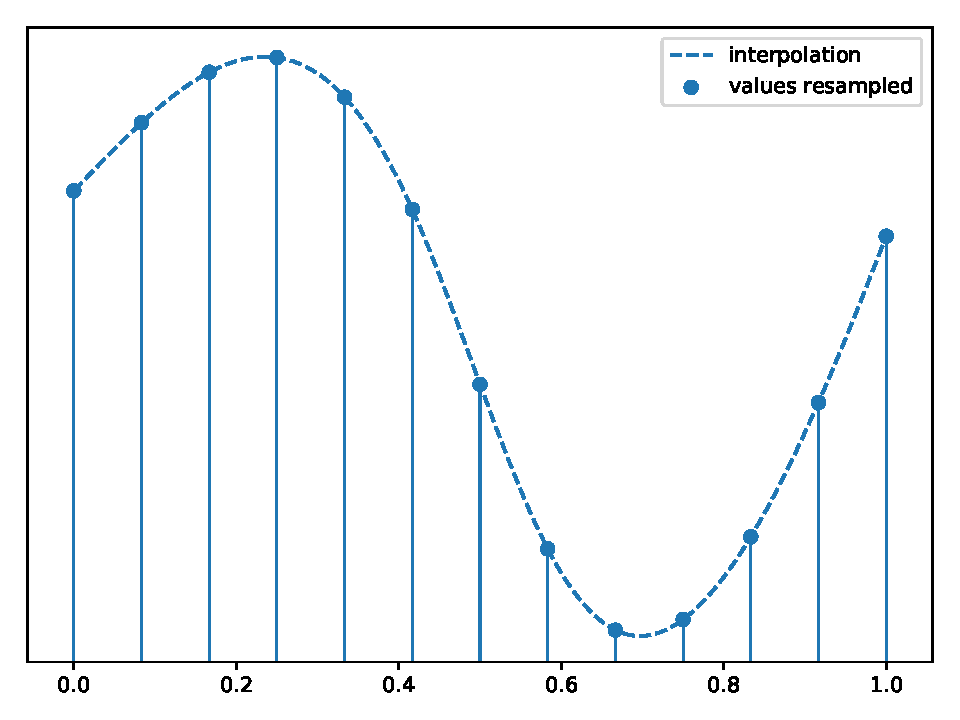
\includegraphics[width=7.5cm]{function-resampled}}
\end{figure}

Although they are not the only methods used for interpolation, splines and
smoothing splines are the most used, for this reason we will focus on them
during this work.
